\apendice{Especificación de Requisitos}

\section{Introducción}

La herramienta Olivia Finder tiene como objetivo principal proporcionar una gestión eficiente de paquetes 
y dependencias de diferentes repositorios, como PyPI, npm, CRAN y Bioconductor. Para lograr esto, hemos 
identificado una serie de requisitos funcionales que guiarán el diseño y la implementación del sistema.

El primer requisito funcional, RF-1, se centra en el almacenamiento eficiente y el acceso rápido a la 
información de paquetes y dependencias. Es fundamental que el sistema pueda almacenar esta información 
de manera eficiente para evitar demoras significativas en la recuperación de datos. Además, el acceso 
rápido a la información permitirá un rendimiento óptimo del sistema.

La extensibilidad y flexibilidad de la estructura de datos es abordada por el requisito RF-2. Dado 
que los repositorios y las relaciones de dependencia pueden evolucionar con el tiempo, es esencial que 
la estructura de datos utilizada sea adaptable y pueda ser modificada o ampliada sin dificultades. Esto 
garantizará que el sistema pueda adaptarse a futuras modificaciones en los repositorios y en las 
necesidades de gestión de dependencias.

El requisito RF-3 se enfoca en la representación específica de paquetes mediante una estructura de 
datos adecuada. Cada paquete debe tener una representación clara y precisa, que incluya los atributos
relevantes para dicho paquete. Esto facilitará la gestión y el análisis de los paquetes y sus dependencias 
dentro del sistema.

El requisito RF-4 se refiere a la representación y exportación genérica de la red de dependencias 
en diferentes formatos. Es importante que la red de dependencias pueda ser representada en formatos 
genéricos de grafo dirigido, así como en otros formatos como diccionarios, listas o dataframes. 
Esta versatilidad en la representación y exportación permitirá un uso más amplio de la red de 
dependencias en diferentes herramientas y análisis.

La reconstrucción de las estructuras de datos a través de la persistencia es abordada por el 
requisito RF-5. El sistema debe ser capaz de reconstruir las estructuras de datos utilizadas 
para almacenar la información de paquetes y dependencias a partir de una forma persistente, como 
archivos o bases de datos. Esto garantizará la integridad de los datos y facilitará la continuidad 
del trabajo en caso de interrupciones o reinicios del sistema.

El requisito RF-6 se centra en el almacenamiento de datos adicionales sobre la relación de dependencia 
entre los paquetes. Además de las dependencias directas, es importante capturar información adicional, 
como la versión concreta utilizada, para permitir un análisis más completo y detallado de las relaciones
 de dependencia.

El sistema debe ser capaz de obtener datos de manera eficiente desde múltiples fuentes, como se indica 
en el requisito RF-7. Esto incluye la capacidad de leer archivos CSV, acceder a APIs de terceros o 
realizar web scraping para obtener la información necesaria de los repositorios. Esta funcionalidad 
flexible garantizará una amplia variedad de opciones para obtener los datos requeridos por el sistema.

El requisito RF-8 se refiere a la obtención de dependencias transitivas de forma dinámica durante la 
ejecución del sistema. Esto implica obtener tanto las dependencias directas como las dependencias 
indirectas de un paquete en tiempo real. Esta funcionalidad permitirá un análisis más completo de las 
relaciones de dependencia y facilitará la toma de decisiones basada en dichas dependencias.

Por último, el requisito RF-9 se centra en el manejo de excepciones. El sistema debe implementar un 
mecanismo para capturar y manejar adecuadamente situaciones excepcionales que puedan surgir durante su 
ejecución. Esto incluye la generación de mensajes de error claros y la posibilidad de gestionar los 
errores de manera adecuada para minimizar su impacto en la funcionalidad general del sistema.

\section{Catalogo de requisitos funcionales}

\begin{itemize}
    \item \textbf{RF-1: Almacenamiento eficiente y acceso rápido a la información de paquetes y dependencias}: 
	
	El sistema debe ser capaz de almacenar la información de manera eficiente y permitir un acceso rápido a los paquetes y sus dependencias, evitando demoras significativas.
    
    \item \textbf{RF-2: Extensibilidad y flexibilidad de la estructura de datos para futuras modificaciones}: 
	
	La estructura de datos utilizada para representar los paquetes y dependencias debe ser flexible y adaptable, de modo que pueda ser modificada o ampliada en el futuro sin dificultades.
    
    \item \textbf{RF-3: Representación específica de paquetes mediante una estructura de datos adecuada}: 
	
	Cada paquete debe tener una representación clara y precisa mediante una estructura de datos que contenga los atributos relevantes para dicho paquete.
    
    \item \textbf{RF-4: Representación y exportación genérica de la red de dependencias en diferentes formatos}: 
	
	La red de dependencias debe poder ser representada y exportada en formatos genéricos de grafo dirigido, así como en otros formatos como diccionario, listas o dataframes, permitiendo una mayor versatilidad en su uso.
    
    \item \textbf{RF-5: Reconstrucción de estructuras de datos a través de la persistencia}: 
	
	El sistema debe ser capaz de reconstruir las estructuras de datos utilizadas para almacenar la información de paquetes y dependencias a partir de una forma persistente, como archivos o bases de datos.
    
    \item \textbf{RF-6: Almacenamiento de datos adicionales sobre la relación de dependencia}: 
	
	Se requiere la capacidad de almacenar información adicional sobre la relación de dependencia entre los paquetes, como la versión concreta utilizada, para capturar detalles específicos y permitir un análisis más completo.
    
    \item \textbf{RF-7: Obtención eficiente de datos desde múltiples fuentes}: 
	
	El sistema debe ser capaz de obtener datos de manera eficiente desde diversas fuentes, como archivos CSV, APIs de terceros o mediante web scraping, permitiendo una amplia variedad de opciones para obtener la información necesaria.
    
    \item \textbf{RF-8: Obtención de dependencias transitivas dinámicamente en tiempo de ejecución}: 
	
	Se debe permitir la obtención de dependencias transitivas de un paquete de forma dinámica durante la ejecución del sistema, lo que implica obtener las dependencias directas e indirectas de un paquete en tiempo real.
    
    \item \textbf{RF-9: Manejo de excepciones para capturar y manejar situaciones excepcionales}: 
	
	El sistema debe implementar un mecanismo para capturar y manejar adecuadamente las situaciones excepcionales que puedan ocurrir durante su ejecución, proporcionando información clara sobre los fallos y permitiendo una gestión adecuada de los errores.
\end{itemize}

\section{Catalogo de requisitos no funcionales}

\begin{itemize}
	\item \textbf{RNF-1 Usabilidad:}
	 
	Es necesario que la biblioteca proporcione a los usuarios una manera sencilla y 
	bien documentada de obtener redes de dependencia. Esto implica aplicar principios, mecanismos y sistemas de organización 
	de código ampliamente utilizados en el lenguaje, de modo que la interfaz de la biblioteca se adapte a la experiencia, 
	las expectativas y los modelos mentales de los usuarios.

	\item \textbf{RNF-2 Rendimiento:} 
	
	Las funciones de la biblioteca deben tener la capacidad de ejecutarse de manera eficiente 
	en equipos domésticos, incluso al trabajar con redes grandes. Se considerará como un caso de prueba el rendimiento del software 
	al operar con la red de paquetes npm (Node.js). El objetivo principal de este requisito es permitir un uso ágil e interactivo, 
	facilitando la exploración y la investigación, y también asegurando que la biblioteca pueda ser aprovechada por una amplia gama 
	de usuarios, que incluyen gestores de repositorios centralizados, desarrolladores de software y desarrolladores de herramientas 
	de calidad continua.

	\item \textbf{RNF-3 Mantenimiento y extensibilidad:} 
	
	El diseño de la biblioteca debe estar orientado a facilitar el mantenimiento 
	correctivo y evolutivo. Esto implica adoptar una estructura y una arquitectura que permitan realizar modificaciones y expansiones 
	de manera eficiente, sin ocasionar interrupciones significativas en el funcionamiento del software.
	
	\item \textbf{RNF-4 Documentación:} 
	
	Es fundamental que la solución esté adecuadamente documentada. Con el propósito de facilitar 
	su divulgación, toda la documentación será redactada en inglés. Esto incluye la inclusión de documentación en el código mediante 
	el uso de docstrings, siguiendo estándares comunes en este aspecto, así como la provisión de ejemplos prácticos que ilustren el 
	uso de las funciones de la biblioteca.
	
	\item \textbf{RNF-5 Soporte:} 
	
	La biblioteca debe ser compatible con versiones de Python superiores a la 3.8. Esto garantiza que 
	la biblioteca pueda ser utilizada en entornos actuales y futuros basados en Python, asegurando así su viabilidad y utilidad a 
	largo plazo.
\end{itemize}

\section{Casos de uso}

Los casos de uso son una técnica para capturar los requisitos funcionales de un sistema. Se trata de una 
descripción de las acciones que realiza un usuario y las respuestas del sistema ante dichas acciones. 
Los casos de uso se representan mediante diagramas de casos de uso, que muestran las relaciones entre los distintos actores y casos de uso del sistema.

A continuacion presentamos los casos de uso del sistema, que se han agrupado en dos grupos: casos de uso de la biblioteca y casos de uso de los notebooks.

\subsection{Casos de uso de la biblioteca}

Los casos de uso de la biblioteca se muestran representados en un diagrama de casos de uso en la figura \ref{fig:casos_de_uso}. 
Los actores que interactúan con el sistema son el usuario y los repositorios de paquetes.

\begin{figure}[h]
	\centering
	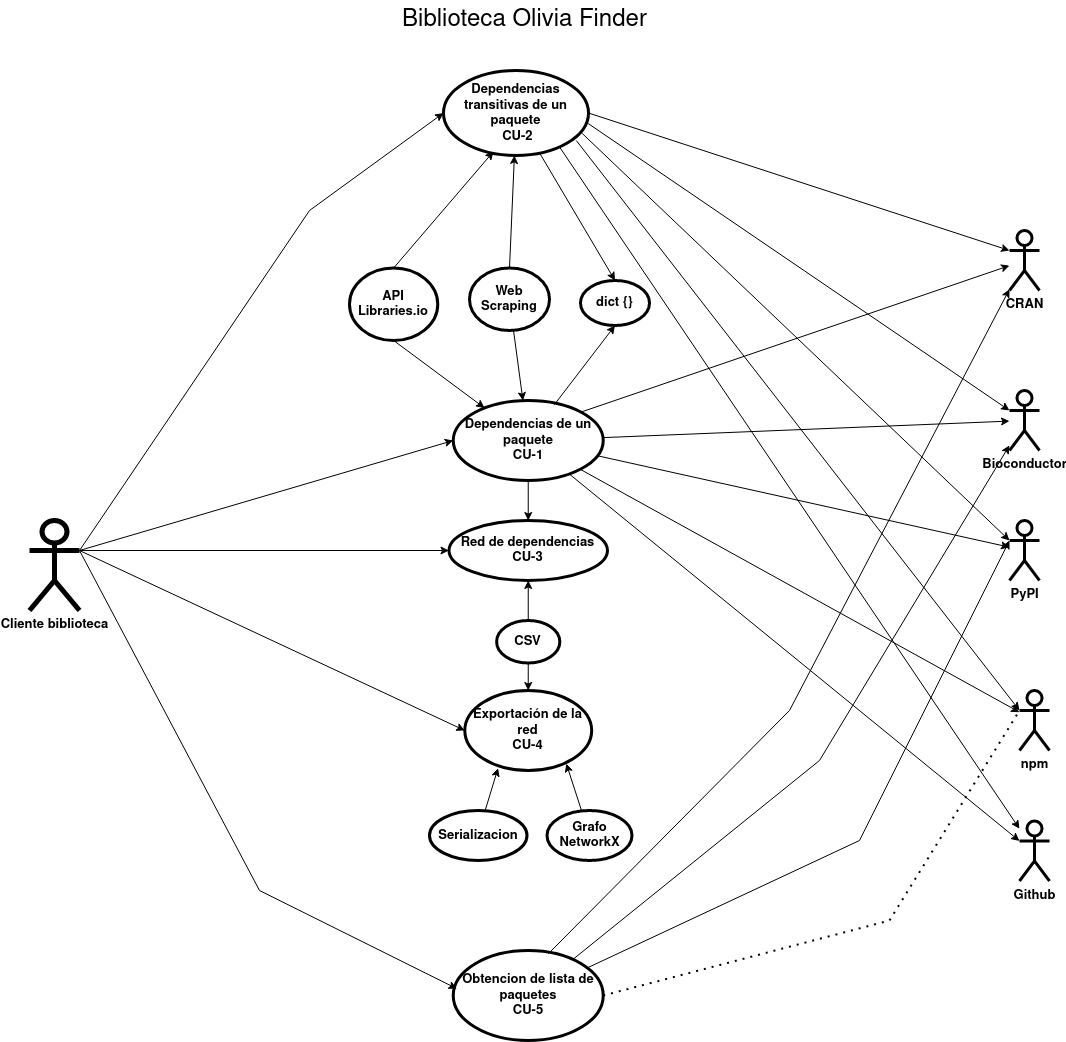
\includegraphics[width=1\textwidth]{img/anexos/Casos_uso_biblioteca.drawio.png}
	\caption{Diagrama de casos de uso de la biblioteca Olivia Finder.}
	\label{fig:casos_de_uso}
\end{figure}

A continuacon se describen los casos de uso de la biblioteca. Cada caso de uso se describe mediante una tabla de las siguientes. \ref{tab:cu1} \ref{tab:cu2} \ref{tab:cu3} \ref{tab:cu4}

\begin{table}[p]
	\centering
	\begin{tabularx}{\linewidth}{ p{0.21\columnwidth} p{0.71\columnwidth} }
		\toprule
		\textbf{CU-1}    & \textbf{Obtención de las ependencias de un paquete}\\
		\toprule
		\textbf{Versión}              & 1.0    \\
		\textbf{Autor}                & Daniel Alonso \\
		\textbf{Requisitos asociados} & RF-1, RF-2, RF-3, RF-6, RF-7, RF-8, RF-9 \\
		\textbf{Descripción}          & Obtener las dependencias de un paquete de las redes 
										PyPI, npm, CRAN, Bioconductor y GitHub. \\
		\textbf{Precondición}         & Las fuentes de datos usadas para obtener las dependencias 
										deben de estar accesibles. \\
		\textbf{Acciones}             &
		\begin{enumerate}
			\def\labelenumi{\arabic{enumi}.}
			\tightlist
			\item Identificar el paquete del cual se desean obtener las dependencias.
			\item Realizar una búsqueda en la fuente de datos para obtener las dependencias del paquete.
		\end{enumerate}\\
		\textbf{Postcondición}        & Se obtienen las dependencias del paquete en formato diccionario. \\
		\textbf{Excepciones}          & Si el paquete no existe en alguna de las redes, se obtiene un diccionario vacío.\\
		\textbf{Importancia}          & Media \\
		\bottomrule
	\end{tabularx}
	\caption{CU-1 Dependencias de un paquete.}
	\label{tab:cu1}
\end{table}

\begin{table}[p]
	\centering
	\begin{tabularx}{\linewidth}{ p{0.21\columnwidth} p{0.71\columnwidth} }
		\toprule
		\textbf{CU-2}    & \textbf{Obtención de las dependencias transitivas de un paquete}\\
		\toprule
		\textbf{Versión}              & 1.0    \\
		\textbf{Autor}                & Daniel Alonso \\
		\textbf{Requisitos asociados} & RF-1, RF-3, RF-7, RF-8, RF-9 \\
		\textbf{Descripción}          & Obtener las dependencias transitivas de un paquete, utilizando una profundidad de búsqueda específica. \\
		\textbf{Precondición}         & Las dependencias directas del paquete están disponibles y las fuentes de datos son accesibles. \\
		\textbf{Acciones}             &
		\begin{enumerate}
			\def\labelenumi{\arabic{enumi}.}
			\tightlist
			\item Identificar el paquete del cual se desean obtener las dependencias transitivas.
			\item Establecer la profundidad de búsqueda deseada.
			\item Recorrer recursivamente las dependencias directas del paquete hasta alcanzar la profundidad de búsqueda establecida.
			\item Registrar todas las dependencias transitivas encontradas durante el recorrido.
		\end{enumerate}\\
		\textbf{Postcondición}        & Se obtienen las dependencias transitivas del paquete hasta la profundidad de búsqueda especificada. \\
		\textbf{Excepciones}          & Si el paquete no existe en las redes de paquetes, se añade como un diccionario vacio.\\
		\textbf{Importancia}          & Media \\
		\bottomrule
	\end{tabularx}
	\caption{CU-2 Dependencias transitivas de un paquete.}
	\label{tab:cu2}
\end{table}


\begin{table}[p]
	\centering
	\begin{tabularx}{\linewidth}{ p{0.21\columnwidth} p{0.71\columnwidth} }
		\toprule
		\textbf{CU-3}    & \textbf{Generación de la red de dependencias de un repositorio}\\
		\toprule
		\textbf{Versión}              & 1.0    \\
		\textbf{Autor}                & Daniel Alonso \\
		\textbf{Requisitos asociados} & RF-3, RF-5, RF-6, RF-7, RF-9 \\
		\textbf{Descripción}          & Generar la red de dependencias de paqutes para un repositorio. \\
		\textbf{Precondición}         & Los repositorios PyPI, npm, CRAN y Bioconductor están accesibles via Web o disponemos de otra fuente de datos soportada. \\
		\textbf{Acciones}             &
		\begin{enumerate}
			\def\labelenumi{\arabic{enumi}.}
			\tightlist
			\item Obtener la lista de paquetes disponibles en el repositorio.
			\item Para cada paquete, obtener sus dependencias directas.
			\item Construir la red de dependencias, donde los paquetes son los nodos y las relaciones de dependencia son los enlaces.
		\end{enumerate}\\
		\textbf{Postcondición}        & Se genera la red de dependencias que muestra las relaciones entre los paquetes en el repositorio. \\
		\textbf{Excepciones}          & Si no es posible acceder a alguno de los repositorios, se obtiene una excepcion.\\
		\textbf{Importancia}          & Alta\\
		\bottomrule
	\end{tabularx}
	\caption{CU-3 Red de dependencias.}
	\label{tab:cu3}
\end{table}

\begin{table}[p]
	\centering
	\begin{tabularx}{\linewidth}{ p{0.21\columnwidth} p{0.71\columnwidth} }
		\toprule
		\textbf{CU-4}    & \textbf{Exportación de la red de dependencias}\\
		\toprule
		\textbf{Versión}              & 1.0    \\
		\textbf{Autor}                & Daniel Alonso \\
		\textbf{Requisitos asociados} & RF-3, RF-4, RF-6 \\
		\textbf{Descripción}          & Almacenar la red de dependencias para su uso posterior por otras herramientas o análisis, asegurando la compatibilidad con la biblioteca OLIVIA. \\
		\textbf{Precondición}         & Se ha generado la red de dependencias correctamente. \\
		\textbf{Acciones}             &
		\begin{enumerate}
			\def\labelenumi{\arabic{enumi}.}
			\tightlist
			\item Exportar la red de dependencias en un formato compatible con la biblioteca OLIVIA.
			\item Guardar el archivo de exportación en una ubicación adecuada para su uso posterior.
		\end{enumerate}\\
		\textbf{Postcondición}        & La red de dependencias se almacena en un formato compatible con la biblioteca OLIVIA para su posterior utilización. \\
		\textbf{Excepciones}          & \\
		\textbf{Importancia}          & Alta \\
		\bottomrule
	\end{tabularx}
	\caption{CU-4 Exportación de la red.}
	\label{tab:cu4}
\end{table}


\subsection{Casos de uso de los notebooks}

\section{Objetivos generales}

% \section{Catálogo de requisitos}

% \section{Especificación de requisitos}





